\documentclass{standalone}
\usepackage{tikz}
\usetikzlibrary{patterns, positioning}


\begin{document}
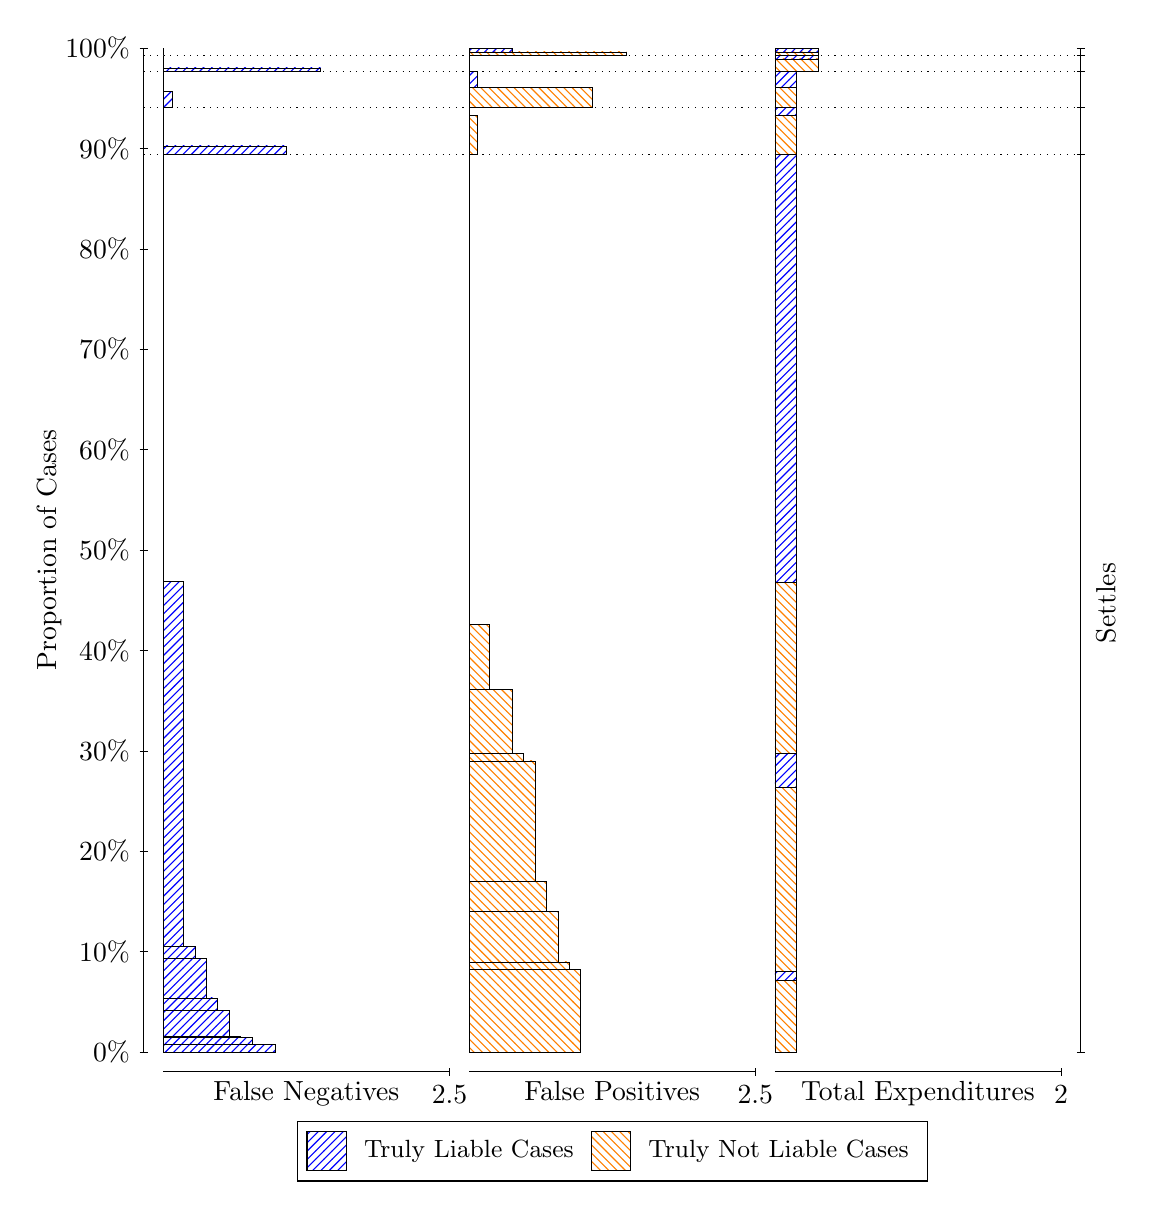
\begin{tikzpicture}
\draw[black, very thin] (1.5,1.75) -- (1.5,14.5);
\node[rotate=90, text=black, anchor=center] at (0.3, 8.125) {Proportion of Cases};
\draw[black, very thin] (1.45,1.75) -- (1.55,1.75);
\node[text=black, anchor=east] at (1.45, 1.75) {0\%};
\draw[black, very thin] (1.45,3.025) -- (1.55,3.025);
\node[text=black, anchor=east] at (1.45, 3.025) {10\%};
\draw[black, very thin] (1.45,4.3) -- (1.55,4.3);
\node[text=black, anchor=east] at (1.45, 4.3) {20\%};
\draw[black, very thin] (1.45,5.575) -- (1.55,5.575);
\node[text=black, anchor=east] at (1.45, 5.575) {30\%};
\draw[black, very thin] (1.45,6.85) -- (1.55,6.85);
\node[text=black, anchor=east] at (1.45, 6.85) {40\%};
\draw[black, very thin] (1.45,8.125) -- (1.55,8.125);
\node[text=black, anchor=east] at (1.45, 8.125) {50\%};
\draw[black, very thin] (1.45,9.4) -- (1.55,9.4);
\node[text=black, anchor=east] at (1.45, 9.4) {60\%};
\draw[black, very thin] (1.45,10.675) -- (1.55,10.675);
\node[text=black, anchor=east] at (1.45, 10.675) {70\%};
\draw[black, very thin] (1.45,11.95) -- (1.55,11.95);
\node[text=black, anchor=east] at (1.45, 11.95) {80\%};
\draw[black, very thin] (1.45,13.225) -- (1.55,13.225);
\node[text=black, anchor=east] at (1.45, 13.225) {90\%};
\draw[black, very thin] (1.45,14.5) -- (1.55,14.5);
\node[text=black, anchor=east] at (1.45, 14.5) {100\%};

\draw[black, very thin] (13.4,1.75) -- (13.4,14.5);
\draw[black, very thin] (13.35,1.75) -- (13.45,1.75);
\node[anchor=west] at (13.35, 1.75) {};
\draw[black, very thin] (13.35,13.152) -- (13.45,13.152);
\node[anchor=west] at (13.35, 13.152) {};
\draw[black, very thin] (13.35,13.75) -- (13.45,13.75);
\node[anchor=west] at (13.35, 13.75) {};
\draw[black, very thin] (13.35,14.204) -- (13.45,14.204);
\node[anchor=west] at (13.35, 14.204) {};
\draw[black, very thin] (13.35,14.407) -- (13.45,14.407);
\node[anchor=west] at (13.35, 14.407) {};
\draw[black, very thin] (13.35,14.5) -- (13.45,14.5);
\node[anchor=west] at (13.35, 14.5) {};

\draw[black, very thin, pattern color=blue, pattern=north east lines] (1.75,1.75) rectangle (3.167,1.8447);
\draw[black, very thin, pattern color=blue, pattern=north east lines] (1.75,1.8447) rectangle (2.8763,1.9379);
\draw[black, very thin, pattern color=blue, pattern=north east lines] (1.75,1.9379) rectangle (2.731,1.9522);
\draw[black, very thin, pattern color=blue, pattern=north east lines] (1.75,1.9522) rectangle (2.5857,2.2815);
\draw[black, very thin, pattern color=blue, pattern=north east lines] (1.75,2.2815) rectangle (2.4403,2.4381);
\draw[black, very thin, pattern color=blue, pattern=north east lines] (1.75,2.4381) rectangle (2.295,2.9384);
\draw[black, very thin, pattern color=blue, pattern=north east lines] (1.75,2.9384) rectangle (2.1497,3.0951);
\draw[black, very thin, pattern color=blue, pattern=north east lines] (1.75,3.0951) rectangle (2.0043,7.7241);
\draw[black, very thin, pattern color=orange, pattern=north west lines] (1.75,7.7241) rectangle (1.75,13.152);
\draw[black, very thin, pattern color=blue, pattern=north east lines] (1.75,13.152) rectangle (3.3123,13.256);
\draw[black, very thin, pattern color=orange, pattern=north west lines] (1.75,13.256) rectangle (1.75,13.75);
\draw[black, very thin, pattern color=blue, pattern=north east lines] (1.75,13.75) rectangle (1.859,13.953);
\draw[black, very thin, pattern color=orange, pattern=north west lines] (1.75,13.953) rectangle (1.75,14.204);
\draw[black, very thin, pattern color=blue, pattern=north east lines] (1.75,14.204) rectangle (3.7483,14.248);
\draw[black, very thin, pattern color=orange, pattern=north west lines] (1.75,14.248) rectangle (1.75,14.407);
\draw[black, very thin, pattern color=orange, pattern=north west lines] (1.75,14.407) rectangle (1.75,14.45);
\draw[black, very thin, pattern color=blue, pattern=north east lines] (1.75,14.45) rectangle (1.75,14.5);
\draw[black, very thin, pattern color=orange, pattern=north west lines] (5.6333,1.75) rectangle (7.0503,2.7992);
\draw[black, very thin, pattern color=orange, pattern=north west lines] (5.6333,2.7992) rectangle (6.905,2.8941);
\draw[black, very thin, pattern color=orange, pattern=north west lines] (5.6333,2.8941) rectangle (6.7597,3.5393);
\draw[black, very thin, pattern color=orange, pattern=north west lines] (5.6333,3.5393) rectangle (6.6143,3.9213);
\draw[black, very thin, pattern color=orange, pattern=north west lines] (5.6333,3.9213) rectangle (6.469,5.4465);
\draw[black, very thin, pattern color=orange, pattern=north west lines] (5.6333,5.4465) rectangle (6.3237,5.5388);
\draw[black, very thin, pattern color=orange, pattern=north west lines] (5.6333,5.5388) rectangle (6.1783,6.3585);
\draw[black, very thin, pattern color=orange, pattern=north west lines] (5.6333,6.3585) rectangle (5.8877,7.1777);
\draw[black, very thin, pattern color=blue, pattern=north east lines] (5.6333,7.1777) rectangle (5.6333,13.152);
\draw[black, very thin, pattern color=orange, pattern=north west lines] (5.6333,13.152) rectangle (5.7423,13.646);
\draw[black, very thin, pattern color=blue, pattern=north east lines] (5.6333,13.646) rectangle (5.6333,13.75);
\draw[black, very thin, pattern color=orange, pattern=north west lines] (5.6333,13.75) rectangle (7.1957,14.001);
\draw[black, very thin, pattern color=blue, pattern=north east lines] (5.6333,14.001) rectangle (5.7423,14.204);
\draw[black, very thin, pattern color=orange, pattern=north west lines] (5.6333,14.204) rectangle (5.6333,14.363);
\draw[black, very thin, pattern color=blue, pattern=north east lines] (5.6333,14.363) rectangle (5.6333,14.407);
\draw[black, very thin, pattern color=orange, pattern=north west lines] (5.6333,14.407) rectangle (7.6317,14.45);
\draw[black, very thin, pattern color=blue, pattern=north east lines] (5.6333,14.45) rectangle (6.1783,14.5);
\draw[black, very thin, pattern color=orange, pattern=north west lines] (9.5167,1.75) rectangle (9.7892,2.662);
\draw[black, very thin, pattern color=blue, pattern=north east lines] (9.5167,2.662) rectangle (9.7892,2.7695);
\draw[black, very thin, pattern color=orange, pattern=north west lines] (9.5167,2.7695) rectangle (9.7892,5.1139);
\draw[black, very thin, pattern color=blue, pattern=north east lines] (9.5167,5.1139) rectangle (9.7892,5.5379);
\draw[black, very thin, pattern color=orange, pattern=north west lines] (9.5167,5.5379) rectangle (9.7892,7.7092);
\draw[black, very thin, pattern color=blue, pattern=north east lines] (9.5167,7.7092) rectangle (9.7892,13.152);
\draw[black, very thin, pattern color=orange, pattern=north west lines] (9.5167,13.152) rectangle (9.7892,13.646);
\draw[black, very thin, pattern color=blue, pattern=north east lines] (9.5167,13.646) rectangle (9.7892,13.75);
\draw[black, very thin, pattern color=orange, pattern=north west lines] (9.5167,13.75) rectangle (9.7892,14.001);
\draw[black, very thin, pattern color=blue, pattern=north east lines] (9.5167,14.001) rectangle (9.7892,14.204);
\draw[black, very thin, pattern color=orange, pattern=north west lines] (9.5167,14.204) rectangle (10.062,14.363);
\draw[black, very thin, pattern color=blue, pattern=north east lines] (9.5167,14.363) rectangle (10.062,14.407);
\draw[black, very thin, pattern color=orange, pattern=north west lines] (9.5167,14.407) rectangle (10.062,14.45);
\draw[black, very thin, pattern color=blue, pattern=north east lines] (9.5167,14.45) rectangle (10.062,14.5);
\draw[black, dotted] (1.5,13.152) -- (13.4,13.152);
\draw[black, dotted] (1.5,13.75) -- (13.4,13.75);
\draw[black, dotted] (1.5,14.204) -- (13.4,14.204);
\draw[black, dotted] (1.5,14.407) -- (13.4,14.407);
\draw[black, very thin] (1.75,1.5) -- (5.3833,1.5);
\node[text=black, anchor=north] at (3.5667, 1.5) {False Negatives};
\draw[black, very thin] (5.3833,1.45) -- (5.3833,1.55);
\node[text=black, anchor=north] at (5.3833, 1.45) {2.5};

\draw[black, very thin] (5.6333,1.5) -- (9.2667,1.5);
\node[text=black, anchor=north] at (7.45, 1.5) {False Positives};
\draw[black, very thin] (9.2667,1.45) -- (9.2667,1.55);
\node[text=black, anchor=north] at (9.2667, 1.45) {2.5};

\draw[black, very thin] (9.5167,1.5) -- (13.15,1.5);
\node[text=black, anchor=north] at (11.333, 1.5) {Total Expenditures};
\draw[black, very thin] (13.15,1.45) -- (13.15,1.55);
\node[text=black, anchor=north] at (13.15, 1.45) {2};

\node[text=black, centered, rotate=90] at (13.72, 7.4509) {Settles};





\draw (7.449999999999999,1.5) node[draw=none] (baseCoordinate) {};
\begin{scope}[align=center]
        \matrix[scale=0.5, draw=black, below=0.5cm of baseCoordinate, nodes={draw}, column sep=0.1cm]{
            \node[rectangle, draw, minimum width=0.5cm, minimum height=0.5cm, pattern color=blue, pattern=north east lines] {}; &
            \node[draw=none, font=\small, text=black] (B) {Truly Liable Cases}; &
            \node[rectangle, draw, minimum width=0.5cm, minimum height=0.5cm, pattern color=orange, pattern=north west lines] {}; &
            \node[draw=none, font=\small, text=black] (B) {Truly Not Liable Cases}; \\
            };
\end{scope}

\end{tikzpicture}
\end{document}